\documentclass[12pt,letterpaper]{article}

\usepackage[
    top=0.8in,
    bottom=0.8in,
    left=0.8in,
    right=0.8in,
    marginparwidth=0mm,
    marginparsep=0mm,
    headheight=15pt,
    centering,
    % showframe,
    includefoot,
    includehead
    ]{geometry}


\usepackage{setspace}
\usepackage{titlesec}
\usepackage{lipsum}
\usepackage{amssymb}
\usepackage{amsmath}
\usepackage{xcolor}
\usepackage{graphicx}
\usepackage[most]{tcolorbox}

\usepackage{blindtext}
\usepackage{multicol}
\usepackage{fancyhdr}

% the root directory of all of our images
\graphicspath{ {./img/} }

\definecolor{alggrey}{rgb}{0.94,0.94,0.94}

% \colorlet{LightLavender}{Lavender!40!}
\tcbset{
  on line, 
  boxsep=4pt, left=0pt,right=0pt,top=0pt,bottom=0pt,
  colframe=white, colback=alggrey,  
  highlight math style={enhanced}
}

%----------------------------------------------------------------------------------------
%	Format of Sections
%----------------------------------------------------------------------------------------
\titleformat{\section}
    {\Huge\sc}{\thesection{}. }{0.2em}{}
\titlespacing{\section}{0pc}{*4}{*1.5}

\titleformat{\subsection}
    {\Large\bfseries}{}{0.0em}{\sc\thesubsection{}. }
\titlespacing{\subsection}{0pc}{*4}{*1.5}

\titleformat{\subsubsection}
    {\large}{}{0em}{\thesubsubsection{}. }
\titlespacing{\subsubsection}{0pc}{*4}{*1.5}

%----------------------------------------------------------------------------------------





%----------------------------------------------------------------------------------------
%	Header & Footer
%----------------------------------------------------------------------------------------
\pagestyle{fancy}
\fancyhf{}
\lhead{Solving the Rubik's Cube}
\rhead{Ga\"etan Almela}
\rfoot{\thepage}
\renewcommand{\headrulewidth}{0pt}

%----------------------------------------------------------------------------------------






%----------------------------------------------------------------------------------------
%	New Commands
%----------------------------------------------------------------------------------------
\newcommand{\TODO}{\color{red}\textbf{TODO}\color{black}}

% create a command to display examples in a box
\newcommand{\note}[1]{
    \medskip \noindent
    \fcolorbox{lightgray}{white}{
	\parbox[t]{\textwidth}{
	    \textit{\textbf{Note}}: #1
        }
    } 
}

\newcommand{\alg}[1]{
  \tcbox{
    {\tt #1}
  }
}

% shortcut command for pictures
\newcommand{\pic}[1]{
  \begin{center}
	  \includegraphics[scale=0.3]{#1}
  \end{center}
}

% shortcut command for pictures with text
\newcommand{\pictxt}[2]{
  \begin{center}
	  \includegraphics[scale=0.3]{#1}

    {\sc #2}
  \end{center}
}

% shortcut command for notation specifically
\newcommand{\npic}[2]{
  \begin{center}
	  \includegraphics[scale=0.2]{#1}

	  {#2}
  \end{center}
}

%----------------------------------------------------------------------------------------



\doublespacing

\begin{document}

% no header on first page
\thispagestyle{empty}

\topskip0pt
\vspace*{\fill}

\begin{center}
    {\textit{\Huge Solving the Rubik's Cube}}

    \hfill

    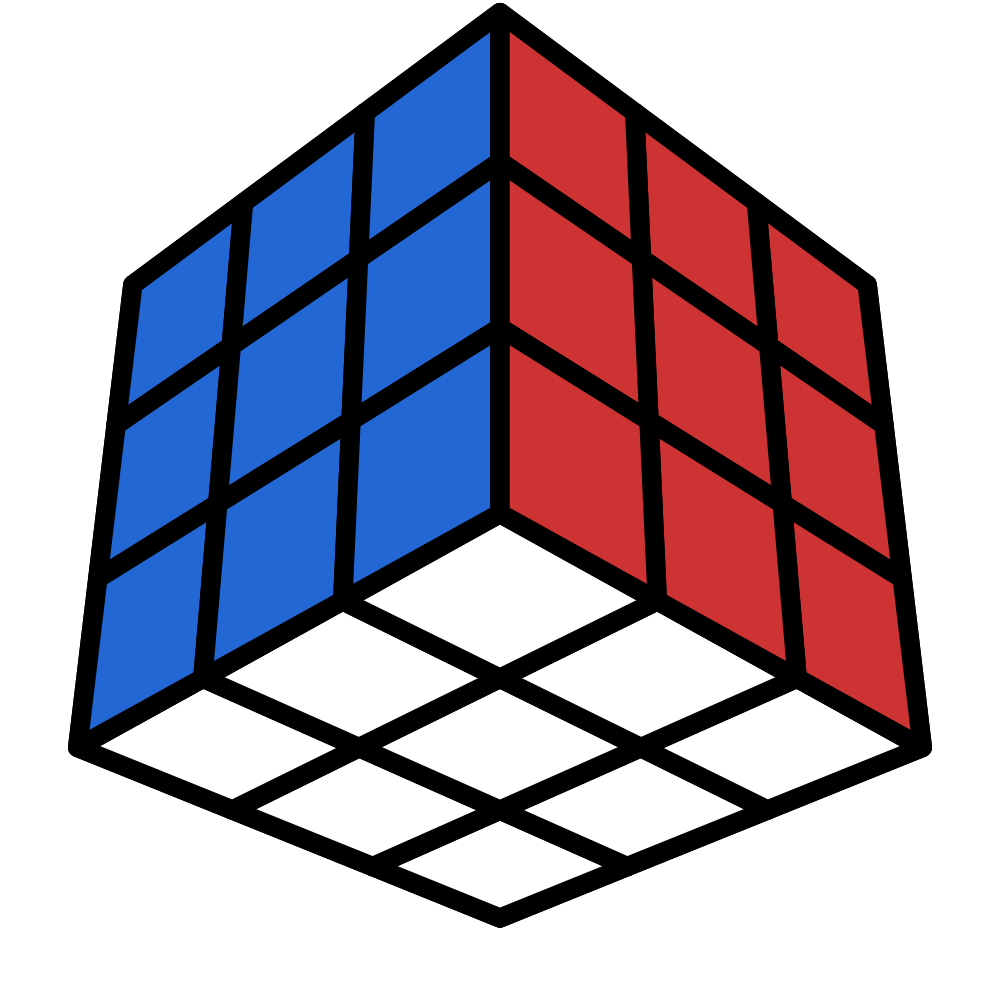
\includegraphics[scale=0.3]{cover}

    \hfill

    {\sc{\Large Ga\"etan Almela}}
\end{center}

\vspace*{\fill}

\newpage

\tableofcontents

\newpage



\section{Introduction}
I first learned to solve a Rubik's cube when I was twelve years old. At the
time, I followed a series of YouTube videos by online creator Dan Brown. My
first attempt took me a few hours, but once it was finally solved, it was
exhilarating. Little could describe the feeling of satisfaction that comes with
solving a Rubik's cube for the first time, a puzzle that is often portrayed by
pop culture as the quintessential brain teaser for geniuses. Spoiler alert: it's
not. In only a couple of days of practice, I was able to consistently solve the
cube in under 3 minutes. I didn't know it at the time, but for the next 8 years
of my life I would become very competitive at strange discipline that is speed
solving the cube.

Today, I can solve a Rubik's cube in about ten seconds; I certainly know much
more about the puzzle than I did at the time. In this instruction manual, I hope
to bring you the same feeling I got when I solved my first cube. Moreover, I
hope to convince you that solving a Rubik's cube is not as hard as you may
imagine, and that given a methodology, anyone can do it. If you're ready to
crack the cube, keep reading.

\newpage


\section{Thinking about the Cube}

Before we can start solving the cube, there are various concepts which will help
us in thinking about the puzzle. It is worth the effort to consider them before
we start solving, as it will make the process smoother as we go on.

\subsection{The Various Types of Pieces}

It is common for beginners to think about the Rubik's cube as a six sides, each
with nine stickers. However this interpretation is actually quite limiting. In
order to solve the cube, it will be better for us to think of the cube not as
uncoordinated stickers, but instead as \textit{interconnected types of pieces}.

Rubik's cubes have three types of pieces: {\sc centers}, {\sc edges}, and
{\sc corners}.

\begin{multicols}{3}
    \pictxt{centers}{The centers}

    \pictxt{edges}{The edges}

    \pictxt{corners}{The corners}
\end{multicols}

It's crucial to note that {\it each piece type will always remain the same}.
That is: centers will always be centers, edges will always be edges, and corners
will always be corners.

Additionally, no matter what moves you make on the cube, {\it the centers will
never move, relative to each other}. This is extremely important, because it
means that we can use the centers of the cube as a reference for how to solve
it.

To solve the cube is to put every piece where it belongs. This may sound
obvious, but how do we know where any piece needs to go? The answer is actually
quite simple: {\bf a piece goes between the centers of its colors}. This is so
important that it is worth considering some examples.

{{\bf Example 1} \textemdash{} Solving an Edge}

Suppose we are solving the cube and we are interested in solving the {\sc blue},
{\sc yellow} edge.

\pic{blue_yellow_unsolved}

\note{
    The grayed-out pieces don't matter, they could be anything and we are not
    interested in them.
}

To solve this piece, we would need to put the {\sc blue}, {\sc yellow} edge
between the {\sc blue} {\sc yellow} centers.

\pic{blue_yellow_solved}

This solves the edge.

{{\bf Example 2} \textemdash{} Solving a Corner}

Suppose we are solving the cube and we are interested in solving the {\sc blue},
{\sc yellow}, {\sc red} corner.

\pic{blue_yellow_red_unsolved}

To solve it, we would need to put the {\sc blue}, {\sc yellow}, {\sc red} corner
between the {\sc blue}, {\sc yellow}, {\sc red} centers.

\pic{blue_yellow_red_solved}

This solves the corner. Notice that a piece can be in the correct {\it
location}, but {\it oriented} incorrectly. This can happen for both corners and
edges.

\note{
    The {\it location} of a piece is where it is on the cube. The {\it
    orientation} of a piece is how it is rotated.
}



Don't worry if not everything makes complete sense at this stage, we will
develop most of this intuition as we solve the cube.


\subsection{The Different Layers}

Another very helpful type of intuition we use in solving the cube is to think
about it in {\it layers}. A standard 3x3 Rubik's cube has three layers: the
first layer, the second layer, and the third layer (most often referred to as
the last layer.)

\begin{multicols}{3}
    \pictxt{first_layer}{The first layer}

    \pictxt{middle_layer}{The middle layer}

    \pictxt{last_layer}{The last layer}
\end{multicols}

We differentiate the layers in this way because we will solve each one slightly
differently. Notice that the first layer is on the {\it bottom}: it is common,
when solving the cube, to maintain one orientation throughout the solve.



% \newpage
\subsection{The Colors Matter}

The last important piece of intuition we need before we can start solving our
first cube is the notion of {\it adjacent} and {\it opposite} colors. This is
arguably the most subjective part of this guide, and you don't absolutely need
to know it, but it can be helpful to know when solving the cube.

On a {\it standard} Rubik's cube, the color scheme is as follows:

\begin{itemize}
    \item {\sc White} opposite {\sc Yellow}
    \item {\sc Blue} opposite {\sc Green}
    \item {\sc Red} opposite {\sc Orange}
\end{itemize}

\note {
    For people with colorblindness, it is common to change {\sc red}
    stickers to {\sc pink}, or some other color to distinguish it from the
    {\sc green}.
}

The two opposite sides of the cube illustrate which colors are adjacent.

\begin{multicols}{2}
    \begin{center}
	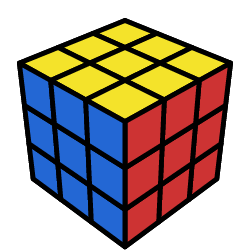
\includegraphics[scale=0.3]{cube_front}
    \end{center}

    \begin{center}
	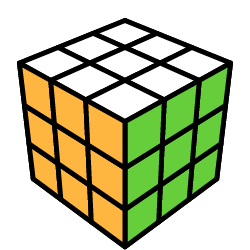
\includegraphics[scale=0.3]{cube_back}
    \end{center}
\end{multicols}

Most cubes you will encounter will follow this color scheme.



\newpage

\section{Notation}

In order to manipulate the cube, people have developed a notation, luckily, it
is quickly learned, and if you forget it, you can simply refer back to this part
of the manual.

There are {\sc six} different types of moves (one for each side) and {\sc
three} different types of rotation (one for each axis) of the cube, each of
which with two variants (clockwise or counter-clockwise.)

In this table, you would be holding the cube with {\sc Yellow} on top, and {\sc
Blue} in front.

% \TODO{} Use table for notation instead?

\newpage

\subsection{Moves}

\begin{multicols}{6}
    \npic{notation/U}{\alg{U}}

    \npic{notation/F}{\alg{F}}

    \npic{notation/R}{\alg{R}}

    \npic{notation/D}{\alg{D}}

    \npic{notation/B}{\alg{B}}

    \npic{notation/L}{\alg{L}}
\end{multicols}

% -------------------

\begin{multicols}{6}
    \npic{notation/U_p}{\alg{U'}}

    \npic{notation/F_p}{\alg{F'}}

    \npic{notation/R_p}{\alg{R'}}

    \npic{notation/D_p}{\alg{D'}}

    \npic{notation/B_p}{\alg{B'}}

    \npic{notation/L_p}{\alg{L'}}
\end{multicols}

\subsection{Rotations}

\begin{multicols}{3}
    \npic{notation/x}{\alg{x}}

    \npic{notation/y}{\alg{y}}

    \npic{notation/z}{\alg{z}}
\end{multicols}

% -------------------

\begin{multicols}{3}
    \npic{notation/x_p}{\alg{x'}}

    \npic{notation/y_p}{\alg{y'}}

    \npic{notation/z_p}{\alg{z'}}
\end{multicols}

% maybe add?
% \subsubsection{Extra Moves}


% considering moving all the edge/corner stuff over here?
% \subsection{How does this actually work?}

\newpage

\section{The First Layer}

It's time to actually solve the Rubik's cube! As mentioned above, we will be
doing this layer by layer. This means that the first step on our journey is to
complete the first layer. There are three major steps to completing the first
layer: building the daisy, building the cross, and inserting the corners. We'll
be sure to take it one step at a time.

\subsection{The Daisy}

The first step on our quest to solve the cube is called the daisy. By the end of
this step, our cube will look like this.

\pic{daisy/daisy}

The goal of this step is to prepare ourselves for the cross, which is often a
difficult step for beginners because the way that it is completed highly depends
on the state of your cube. To resolve this, its good to split up this step into
2 to make it easier.

To complete the daisy, look for all {\sc White} edges, and the {\sc Yellow}
center. Our goal will be to move all of these edges on the yellow face.

Notice that both the other centers and the second stickers on the white edges
are grayed out, this is because they don't matter at this stage. In other words,
you can put any white edge on the yellow side and as long as your stickers match
the ones in the image, you're doing the right thing.

Let us look at some examples,

{\bf Example 1}

\begin{multicols}{2}

  \npic{daisy/edge_1}{(start)}

  \npic{daisy/daisy}{\alg{R}}
  
\end{multicols}


{\bf Example 2}

\begin{multicols}{3}

  \npic{daisy/edge_2_1}{(start)}

  \npic{daisy/edge_2_2}{\alg{U}}

  \npic{daisy/daisy}{\alg{F'}}

\end{multicols}




\subsection{The Cross}

Now that we have our daisy, finishing the cross should be much easier. Pick one
of your {\sc White} edges, and by rotating only the yellow side, align it with
its adjacent center, as shown

\begin{multicols}{2}

  \pic{cross/edge_1}

  \pic{cross/edge_2}

\end{multicols}

Once the edge is aligned, simply rotate the adjacent color's center twice to
place the edge in its final location

\pic{cross/edge_3}

Now repeat this process with the other 3 edges, and rotate your puzzle around:
you should see your cross is fully solved.

\pic{cross/final}



\subsection{Inserting the Corners \label{corner_insert}}

Our goal for this step is to complete the first layer of the cube, all that is
left for us to do here is to insert the corners. By the end of this step, our
cube will look like this.

\pic{first_layer/ex}

\note{We can inspect and rotate the cube at anytime, but keep in mind that when
working on it, the white side should always on the bottom.}

To do this, we first need to find our four {\sc white} corners. We'll focus on
each one at a time.

There are two possibilities for where these corners might be, either in the top
layer or in the bottom layer. We'll look at each case separately to learn how to
deal with each of them.

In either case, you'll find that the algorithm that we perform is the same, so
this should make no difference.

{\bf The Algorithm}

\alg {R U R' U'}

\subsubsection{Top layer corners}

Our goal will be to insert the {\sc white} corners in their respective
positions. The first step is to {\it position the corner above where it
belongs}.

\begin{multicols}{2}

  \pic{first_layer/corner_above_incorrect}

  \pic{first_layer/corner_above}

\end{multicols}

In this case, we picked the {\sc Blue}, {\sc White}, {\sc Red} corner, and
rotated it between the {\sc Red}, and {\sc Blue} centers.

\note{
  The corner currently between the {\sc Blue}, {\sc White}, and {\sc Red} center
  could be any piece, it does not matter to us since it will be pushed out.
}


Now perform the algorithm \alg {R U R' U'}. This should insert the corner in the
correct location. However there is a problem: the corner might be where it
belongs, but it could be {\it misoriented}, as shown below.

\pic{first_layer/corner_under}

To solve this, simply repeat the algorithm in twos until the corner is oriented
correctly. Below is a figure representing the three possible orientations of a
corner.

\begin{multicols}{3}
  \pic{first_layer/sexy_1}

  \pic{first_layer/sexy_2}

  \pic{first_layer/sexy_3}
\end{multicols}

You can repeat this process with any of your top layer corners, keeping in mind
that you are only targeting corners with {\sc White} on them.


\subsubsection{Bottom layer corners}

If a {\sc White} corner is in the bottom layer, simply perform the algorithm
once, this should turn the corner into a top layer corner. You can then simply
follow the instructions for that step.

\begin{multicols}{2}
  \npic{first_layer/bottom_layer_corner_inserted}{Example white corner}

  \npic{first_layer/bottom_layer_corner_out}{After \alg{R U R' U'}}
\end{multicols}

You can repeat this process for each of your bottom layer corners. \\


Once you have repeated the steps described above, your first layer should be
complete! At this stage, you can pat yourself on the back because we are
actually closer to being done than you may think, and the difficult part is largely
behind us. If you are ready to keep going, let's move on to the second layer.



\newpage

\section{The Second Layer}


The second layer might seem daunting, but we actually only need to solve 4
pieces, this is because the centers are already done for us (recall that centers
are always solved relative to each other)

At this step, the only pieces we are looking for are {\it edges with neither
{\sc white} nor {\sc yellow} on them}. We are essentially solving only these
four pieces.

\begin{multicols}{2}

  \pic{second_layer/pieces_1}

  \pic{second_layer/pieces_3}
  
\end{multicols}



The second layer is very algorithmic, which means that we will mostly performing
one algorithm the whole time. To be exact, we will be performing one of two
different algorithms: what we will call the {\it lefty} algorithm and the {\it
righty} algorithm. These algorithms are actually exactly the same, one is simply the
mirror of the other.



\subsection{The Lefty Algorithm}

The lefty algorithm inserts an edge into the left side.

\alg {(U' L' U L) (U F U' F')}

\begin{multicols}{2}

  \pic{second_layer/lefty_edge}

  \pic{second_layer/lefty_solved}

\end{multicols}




\subsection{The Righty Algorithm}

The righty algorithm inserts an edge into the right side.

\alg {(U R U' R') (U' F' U F)}

\begin{multicols}{2}

  \pic{second_layer/righty_edge}

  \pic{second_layer/righty_solved}

\end{multicols}



\note {
  We parenthesize algorithms to make them easier to read. This does not change
  how we actually execute them: we still read them from left to right.
}

{\bf How it works}

What these algorithms allow us to do is to {\it insert} an edge into the middle
layer (what we are working on) without disturbing any of our existing work (i.e.
The bottom layer.) Specifically, these algorithms take the {\it top front} edge,
and insert it either in the {\it front right} or {\it front left} edge


\note {
  As a beginner, it is perfectly normal (and in fact expected) if you don't
  understand how this algorithm works. As you gain more experience with the
  puzzle, you will learn to understand your algorithms much better.
}

\subsection{Solving}

In order to solve the second layer, first identify an edge that doesn't have
{\sc Yellow} or {\sc White} on it. In this case, we'll be solving the {\sc Red}
{\sc Blue} edge.

\pic{second_layer/edge_insert/1}

Next, align this edge with its center

\pic{second_layer/edge_insert/2}

Now you need to figure out if this edge needs to go to the left, or to the
right. To do this, look at the top sticker of the edge, if the matching center
is on the left, perform the lefty algorithm. If the center is on the right,
perform the righty algorithm. In this case, our edge goes on the left

\pic{second_layer/edge_insert/3}

From here, we perform the lefty algorithm, which inserts our edge into its final
location.

\pic{second_layer/edge_insert/4}


\subsubsection{Misinserted Edges}

It's possible at some point throughout this process that an edge you want to
solve will happen to already be in the second layer, but placed or oriented
incorrectly.

\begin{multicols}{2}

  \npic{second_layer/wrong_edge_2}{Incorrect Placement}

  \npic{second_layer/wrong_edge_1}{Incorrect Orientation}
  
\end{multicols}

If this is the case, simply pick a random edge in your top layer, and treat it
as if it belonged in that spot. Then, using the lefty or the righty algorithm,
use it to kick out the edge you want which you can then insert again correctly.
\\

Once you have repeated this process with all four edges, your second layer
should be solved.

\pic{second_layer/f2l}



\newpage

\section{The Last Layer}

We've solved two thirds of our cube! This is a big milestone because at this
stage, the puzzle is solved enough that, by covering the last layer in the palm
of your hand, you could trick somebody into thinking it's completely solved.

If you aren't so interested in these tricks, do not worry as by the end of
this section, we will have completely and honestly solved it. \\

The last layer is unfortunately the most involved part of the solve, and with
good reason: more progress means we need be more careful not to undo our
progress. To do this, we will introduce only {\it two} new algorithms, and a
couple of variations on things we've seen before.

Solving the last layer is done in four steps: (1) orienting the edges, (2)
permuting the edges, (3) permuting the corners, (4) solving the corners. We'll
be sure to take it one step at a time and before we know it, our cube will be
solved.

\subsection{Edge Orientation}

We start solving the last layer by the edges. Our goal in this step will be to
create a {\sc Yellow} cross with all four correctly permuted edges. By the end
of this stage, our cube will look like this.

\pic{last_layer/f2l_cross}

What we want to accomplish in this step is to {\it orient} all edges of the last
layer correctly. More concretely, by the end of this step, we will have our
last layer edges forming a cross on the top layer, as such

\pic{last_layer/f2l_cross_up}

Doing this is surprisingly easy, as we will only be repeating one algorithm until
it is done. The algorithm is as follows

\alg{F (R U R' U') F'}

Notice the \alg{R U R' U'}. This is the same algorithm that we used all the way
back when we were inserting the first layer corners in section
\ref{corner_insert}.

\note{
  This four move algorithm is actually used so often that it has a name: {\it
  the sexy move}.
}

To solve the {\sc Yellow} cross, first look at the edges of your last layer. You
should see one of the following four patterns.

\begin{multicols}{4}

  \pic{last_layer/opt_1}

  \pic{last_layer/opt_2}

  \pic{last_layer/opt_3}

  \pic{last_layer/opt_4}

\end{multicols}

If you already have a cross on the top layer, you can skip this step. If you
don't, first identify which of the following patterns you have in your top
layer, and align it to match with its corresponding case. Next, simply perform the
algorithm once. This should change the shape on your top layer to match another
case shown above. Align it so that it matches the picture, and keep perform the
algorithm again. Keep repeating this process until your cross is fully solved.

\subsection{Edge Permutation}

Next up is to permute the edges. To do this, we'll use a simple algorithm: {\it
the sune}. This again is an algorithm that is so common that it has its own
name. The sune is a great algorithm for plenty of reasons, but for us now, it's
only good for one thing: permuting edges.

The sune algorithm goes as follows

\alg{(R U R') (U R U2 R')}

There are 3 possible cases that we can get at this stage of the puzzle. The
first is that all of our edges are correctly permuted, in which case you can skip this
step! This happens surprisingly often and it's always a nice surprise.

\begin{multicols}{2}

  \pic{last_layer/permutation/correct}

  \pic{last_layer/permutation/correct_3d}

\end{multicols}

If your last layer edge colors match the picture above, (note that you
might need to rotate the layer for your to match) you can skip this step. \\

The second possible case is {\bf the opposite swap}: when two opposite edges
need to swap sides.

\begin{multicols}{2}

  \pic{last_layer/permutation/opposite}

  \pic{last_layer/permutation/opposite_3d}

\end{multicols}

The third and final possibility is {\bf adjacent swap}: when two
adjacent edges need to swap.

\begin{multicols}{2}

  \pic{last_layer/permutation/adjacent}

  \pic{last_layer/permutation/adjacent_3d}

\end{multicols}

\note{
  If you can't identify which of these cases you think you have, rotate the top
  layer and check again, as it my be difficult to spot at first glance.
}

{\bf The Adjacent Swap}

If two adjacent edges of your puzzle need to swap, place the two incorrect edges
in front and to the left as shown, and perform the following algorithm.

\alg{[sune] U}

\begin{multicols}{2}

  \pic{last_layer/permutation/adjacent_setup}

  \pic{last_layer/permutation/adjacent_solved}
  
\end{multicols}

\note{ In the image above, {\sc Red} is treated as the front face. }


{\bf The Opposite Swap}

If two opposite edges of your puzzle need to swap, place the two incorrect edges
in front and in the back (so the side edges of your puzzle should be correct),
and perform the following algorithm:

\alg{[sune] U' [sune]}

\begin{multicols}{2}

  \pic{last_layer/permutation/opposite_setup}

  \pic{last_layer/permutation/opposite_solved}
  
\end{multicols}


\subsection{Corner Permutation}

We've finally solved all of our edges, which means that we're down to the last
four corners of the cube. You can pat yourself on the back for the work you've
done so far; most of the work is behind us. At this stage, there's only one new
algorithm that we're going to need to learn, and I promise that it's easy. After
that, we'll use our good old sexy move to orient our corners and before we know
it, we'll have solved the Rubik's Cube.

To permute the corners, we'll need that new algorithm I was mentioning. This
algorithm has no name, and frankly I've never seen it used at the top level, but
for the sake of this guide, we'll call it {\bf the Pillar's Algorithm}.

{\bf The Pillar's Algorithm}

\alg{U R U' L U R' U' L}

This might look big and scary but I promise that it's easier than you think. The
reason I call this algorithm the pillar's algorithm is because, when you do it,
it looks like two pillars getting broken up and put back together. One pattern
to notice when learning this algorithm is that the top layer always moves back
and forth, and the left and right side alternate.

What this algorithm does is actually very simple: it performs a {\it clockwise
rotation} of the left and back two corners, keeping the front right corner in
place. We'll use it to find a systematic method to permute the corners.

At this stage, you can run into one of two scenarios: the first is that all of
your corners are permuted correctly (in which case you can skip this step), the
second is that one of them is permuted correctly, but the others are not, and
the last is that none of them are permuted correctly.

\note{Be sure to align your edges with their correct sides before evaluating if
your corners are correctly permuted.}

{\bf No correct corners}

If none of your corners are correctly permuted, you can simply perform the
pillars algorithm and check again.

{\bf One correct corner}

If one of your corners is permuted correctly, hold the cube so that the corner
is on the right hand side, and perform the pillars algorithm. At this stage, one
of two things could happen: (1) that correctly permuted all your corners, and
you are done with this step, or (2) your other corners are still not correctly
permuted. If (2) is the case, simply perform the pillars algorithm again, still
with the correct corner in the right hand side, and check again.

By this point, all your corners should be correctly permuted.

\subsection{Corner Orientation}

We've reached the final step on our journey to solve the cube. At the
beginning, you may not have believed that you would solve this thing, but at
this stage, I hope that you believe it more.


For this step, we're going to turn the puzzle around completely, so that the
side that was once our white cross is now facing up. Now a simple but methodical
procedure will follow. If you execute these instructions without fail, I vow
that your puzzle will be solved, however if you make a mistake, you may be set
back quite far in the solving process. As a kid, this was by far the most
stressful step for me, and understandably so: who would want to make a mistake so
close to the end? To make this step easier, we'll break down the process as
much as possible.

{\bf The Procedure}

\begin{enumerate}
  \item Rotate the bottom layer of the cube so that an incorrectly oriented
    corner in the bottom right hand side.
  \item Perform \alg{[sexy]} twice. Recall that \alg{[sexy]} is the algorithm
    that we used all the way back when making our first face: \alg{R U R' U'}.
  \item If the corner is solved but the cube is not fully solved, go to step 1.
    If the corner is not solved, repeat step 2.
\end{enumerate}

At this stage, your cube should be fully solved! If this is your first time
solving a Rubik's Cube, congratulations! It is an honor to me for this guide to
be some people's introduction to the puzzle. I wish you the best in your cubing
adventures.



\newpage

\section{Concluding Thoughts}

If you were able to solve your first Rubik's Cube using this guide,
congratulations, you have achieved something that most people can't say they've
done. I hope that you can see that solving the Rubik's Cube is not necessarily
as hard as you may have imagined. I hope you see that, using the right
procedure, almost anyone can do it. The sense of wonder that comes with solving
a Rubik's Cube is something that I hope to have conveyed to you in this guide,
in the same way that it was conveyed to me when I was younger. With a little
more practice, you should not need to refer to this guide as much and,
eventually, you should no longer need it at all. However you'd be foolish to
think that this is all there is to the cube: some of the top players today use
hundreds of different algorithms to shave off fractions of a second from their
times, and the scene is very competitive. Should you chose to go down this route
of competitive speedcubing, it has been my pleasure to lay down the first brick
on the road of your journey.


\end{document}

